In this module you will learn
\begin{itemize}
	\item what is a solution of a differential equation
	\item the difference between a solution and an integral curve
\end{itemize}

\hfill \\[-10pt]

Assume that we have found a differential equation that models a situation.
Often the goal is to figure out what happens, so we usually attempt to either solve the differential equation and obtain a solution or to find an approximation for the solution.

In this module, we will discuss solutions in more detail.

\begin{definition}[Solution]
	Given a differential equation, a \emph{solution} is a differentiable function that satisfies the differential equation.
\end{definition}

\begin{example}
Consider the differential equation
$$
t \frac{du}{dt} = u + t^2 \cos(t).
$$

Then the function 
$$
u(t) = t\sin(t)
$$
is a solution, because
$$
t \frac{du}{dt} = t \big( \sin(t) + t \cos(t) \big) = t \sin(t) + t^2 \cos (t) = u + t^2 \cos(t).
$$
\end{example}



\begin{definition}[Integral curve]
	We can represent all the solutions geometrically as an infinite family of curves. These curves are called \emph{integral curves}.
\end{definition}

\begin{example}\label{sols-ex}
Consider the initial-value problem
$$
\begin{cases}
	\dfrac{dy}{dx}=-\dfrac{x}{y} \\
	y(0)=-3
\end{cases}
$$
Then, we can check that curves of the form $x^2 + y^2 = C$ satisfy this differential equation.

This gives us the solution
$$
y(x) = - \sqrt{9 - x^2}.
$$

However, the integral curve for this initial-value problem is the curve
$$
x^2 + y^2 = 9
$$


\begin{center}
\begin{tabular}{cc}
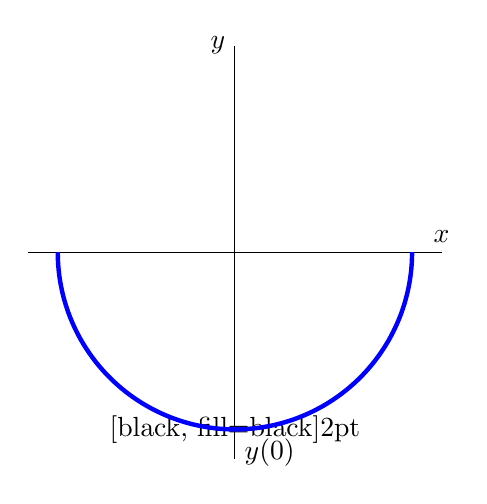
\begin{tikzpicture}[xscale=0.75,yscale=0.75]
	\draw[-{\seta}] (-3.5,0) -- (3.5,0) node[above] {$x$};
	\draw[-{\seta}] (0,-3.5) -- (0,3.5) node[left] {$y$};
	\draw[] (0,-3) node {\tikzcircle[black, fill=black]{2pt}};
	\draw[] (0,-3) node[below right] {$y(0)$};
  \draw[samples=100,ultra thick,domain=0:180,smooth,variable=\t,blue] plot ({3*cos(\t)},{-3*sin(\t)});
\end{tikzpicture}
	& 
	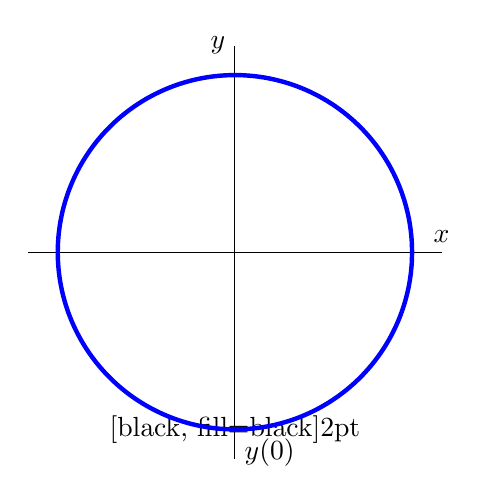
\begin{tikzpicture}[xscale=0.75,yscale=0.75]
		\draw[-{\seta}] (-3.5,0) -- (3.5,0) node[above] {$x$};
		\draw[-{\seta}] (0,-3.5) -- (0,3.5) node[left] {$y$};
		\draw[] (0,-3) node {\tikzcircle[black, fill=black]{2pt}};
		\draw[] (0,-3) node[below right] {$y(0)$};
	  \draw[samples=100,ultra thick,domain=0:360,smooth,variable=\t,blue] plot ({3*cos(\t)},{-3*sin(\t)});
	\end{tikzpicture}

	\\
Solution of the initial-value problem
	& Integral curve for the initial-value problem
\end{tabular}
\end{center}





\end{example}


